% PINO -- physics-informed neural operator.  Build: latexmk -pdf pino.tex
\documentclass[border=8pt]{standalone}
\usepackage{amsmath}
% Shared TikZ palette + node styles for the ML-RT2 architecture diagrams.
% Colours match the ML-RT comparison-paper figures so the three papers look consistent:
%   pink   = data / vectors (inputs, outputs, latent representations)
%   blue   = learned networks / operators (MLPs, encoders, decoders, ...)
%   orange = special operations / physics (spectral transforms, RT residual, ...)
%   green  = loss / training terms
\usepackage{tikz}
\usetikzlibrary{arrows.meta,positioning,fit,backgrounds,calc}

\definecolor{dataFill}{HTML}{F2E6FF}\definecolor{dataDraw}{HTML}{6600CC}
\definecolor{netFill}{HTML}{B5E8E8}\definecolor{netDraw}{HTML}{086565}
\definecolor{opFill}{HTML}{FFE0C2}\definecolor{opDraw}{HTML}{AB4F03}
\definecolor{lossFill}{HTML}{C8F4C1}\definecolor{lossDraw}{HTML}{0C5600}

\tikzset{
  font=\small,
  box/.style  ={draw, rounded corners, align=center, inner sep=4pt, minimum height=9mm, line width=0.3mm},
  data/.style ={box, fill=dataFill, draw=dataDraw},
  net/.style  ={box, fill=netFill,  draw=netDraw},
  op/.style   ={box, fill=opFill,   draw=opDraw},
  loss/.style ={box, fill=lossFill, draw=lossDraw},
  sum/.style  ={draw=netDraw, circle, inner sep=1.3pt, fill=white, line width=0.3mm},
  arr/.style  ={-{Stealth[length=2.4mm]}, thick},
  darr/.style ={-{Stealth[length=2.4mm]}, thick, dashed},
  note/.style ={align=center, font=\scriptsize, text=black!65},
}

\begin{document}
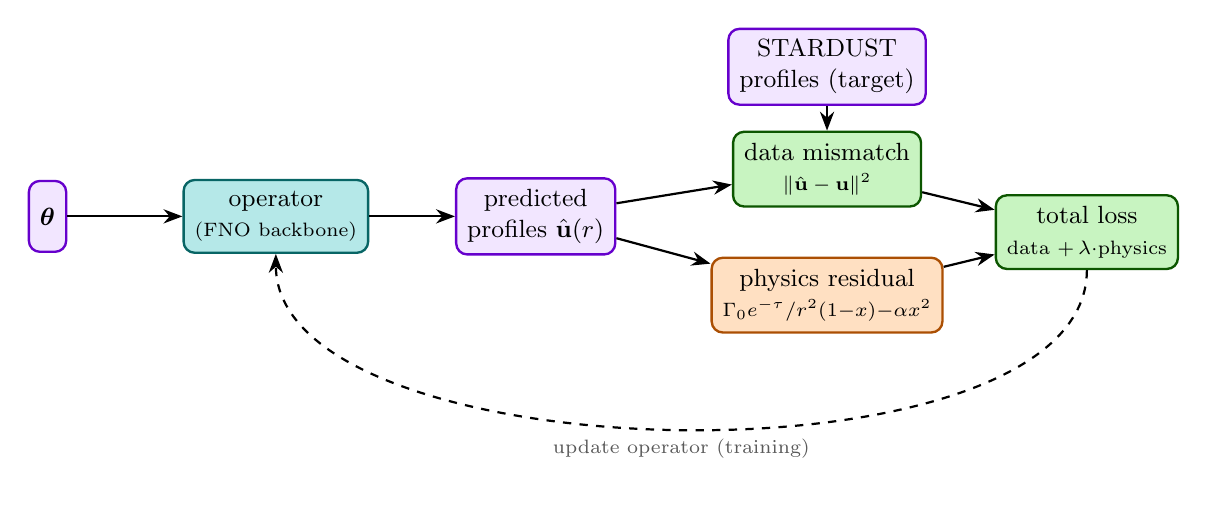
\begin{tikzpicture}
  % main flow: parameters -> operator -> predicted profiles (the OUTPUT)
  \node[data] (th)                        at (0,0)     {$\boldsymbol{\theta}$};
  \node[net,  minimum width=22mm] (op)    at (2.9,0)   {operator\\{\scriptsize (FNO backbone)}};
  \node[data, minimum width=20mm] (pred)  at (6.2,0)   {predicted\\profiles $\hat{\mathbf{u}}(r)$};
  \draw[arr] (th) -- (op);
  \draw[arr] (op) -- (pred);

  % two training terms, both computed from the predicted profiles
  \node[data, minimum width=20mm] (targ)  at (9.9,1.9) {STARDUST\\profiles (target)};
  \node[loss, minimum width=20mm] (dmse)  at (9.9,0.6) {data mismatch\\{\scriptsize $\|\hat{\mathbf u}-\mathbf u\|^2$}};
  \node[op,   minimum width=22mm] (res)   at (9.9,-1.0){physics residual\\{\scriptsize $\Gamma_0 e^{-\tau}/r^2(1{-}x){-}\alpha x^2$}};
  \node[loss, minimum width=18mm] (tot)   at (13.2,-0.2){total loss\\{\scriptsize data $+\,\lambda\cdot$physics}};

  \draw[arr] (targ) -- (dmse);
  \draw[arr] (pred) -- (dmse);
  \draw[arr] (pred) -- (res);
  \draw[arr] (dmse) -- (tot);
  \draw[arr] (res)  -- (tot);
  % training feedback: total loss updates the operator (routed well below everything)
  \draw[darr] (tot.south) to[out=-90,in=-90,looseness=0.7]
        node[below, note] {update operator (training)} (op.south);
\end{tikzpicture}
\end{document}
